\renewcommand{\baselinestretch}{2} \small\normalsize
\chapter{Amplitude Statistics}

\begin{figure}[H]
  \begin{center}
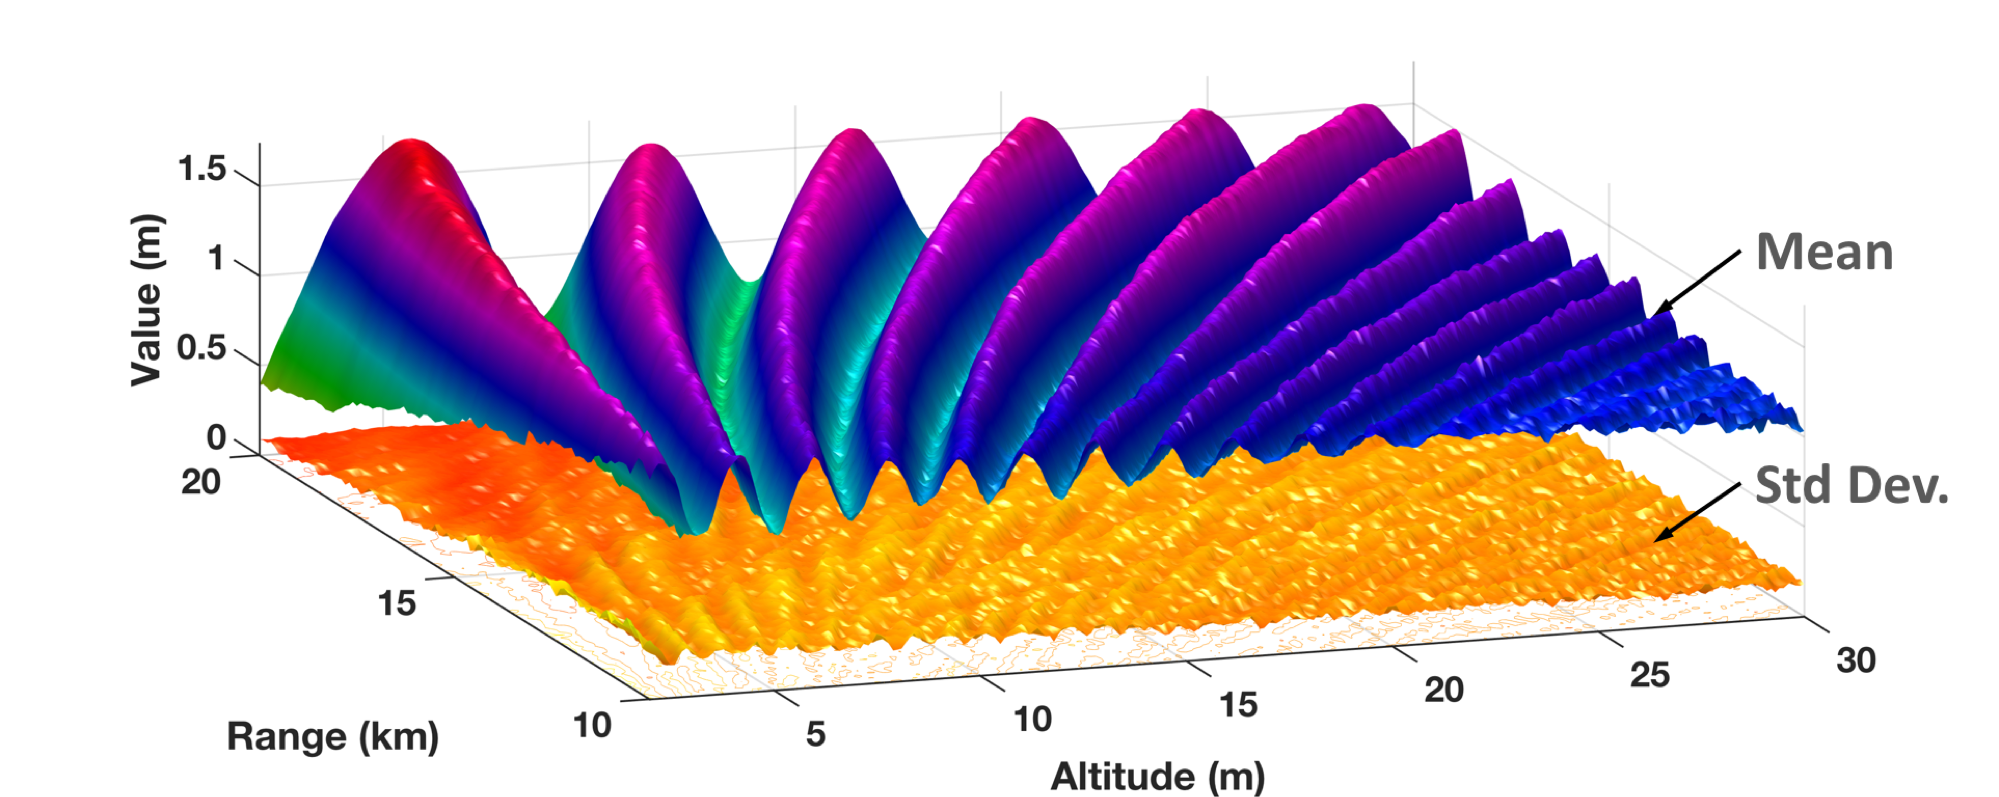
\includegraphics[width=5in]{../media/statistics/ka_band_stats.png}
  \end{center}
  \renewcommand{\baselinestretch}{1} \small\normalsize
  \begin{quote}
    \caption[Ensemble Statistics at Ka-Band]{Ensemble Statistics at Ka-Band\label{stat_fig:1}}
  \end{quote}
\end{figure}
\renewcommand{\baselinestretch}{2} \small\normalsize

\begin{figure}[H]
  \begin{center}
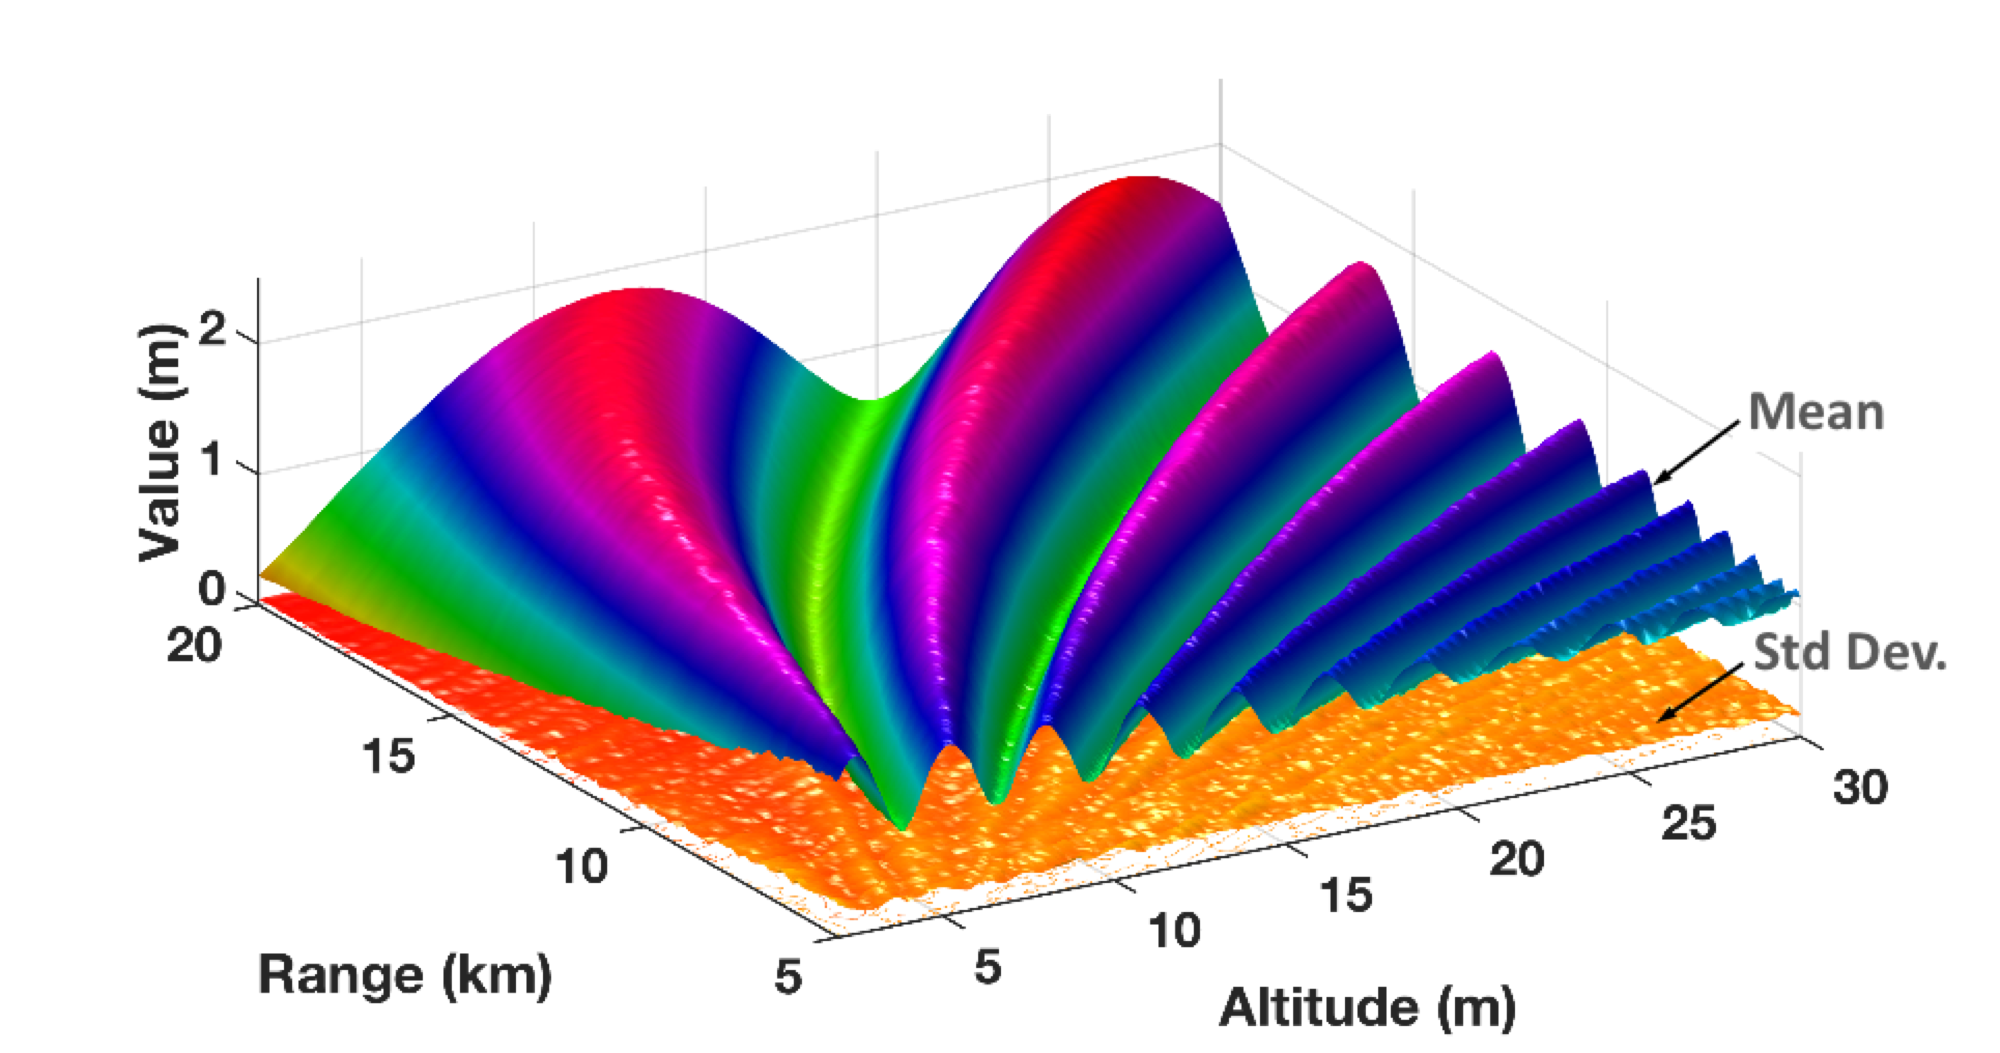
\includegraphics[width=5in]{../media/statistics/x_band_stats.png}
  \end{center}
  \renewcommand{\baselinestretch}{1} \small\normalsize
  \begin{quote}
    \caption[Ensemble Statistics at X-Band]{Ensemble Statistics at X-Band\label{stat_fig:2}}
  \end{quote}
\end{figure}
\renewcommand{\baselinestretch}{2} \small\normalsize

From the propagation factor for the 2 ray model, $F_p = e^{jkL_1} + \Gamma_1e^{jkL_{so}}$, we can look at the phase difference between the two primary paths, $\Delta\varphi = k\left[ L_1 - L_{so}\right]$.
\begin{equation}
\boxed{\Delta\varphi = -\frac{4\pi h_1h_2}{\lambda L}}
\label{stat_eq:1}
\end{equation}
\renewcommand{\baselinestretch}{2} \small\normalsize

\noindent The derivative of the phase difference with respect to range is then
\begin{equation}
\frac{d\Delta\varphi}{dL}=-\frac{4\pi h_1h_2}{\lambda L^2}
\label{stat_eq:2}
\end{equation}

\noindent This can be converted from rad/m to rad/sample by multiplying by the spatial sampling distance in range, $\Delta L$. We can insist that this phase shift per sample be smaller than some pre-determined value to provide adequate sampling. It is often convenient to specify a limit in terms of wavelengths and we can enforce the condition that there must be at least $n$ samples per wavelength by letting

\begin{equation}
\frac{4\pi h_1h_2\Delta L}{\lambda L^2} \leq \frac{2\pi \lambda}{n}
\label{stat_eq:3}
\end{equation}

This yields a constraint for the maximum allowable spatial sampling step to ensure $n$ samples per wavelength.
\begin{equation}
\boxed{\Delta L \leq \frac{\lambda^2 L^2}{2nh_1h_2}}
\label{stat_eq:4}
\end{equation}

\begin{figure}[H]
  \begin{center}
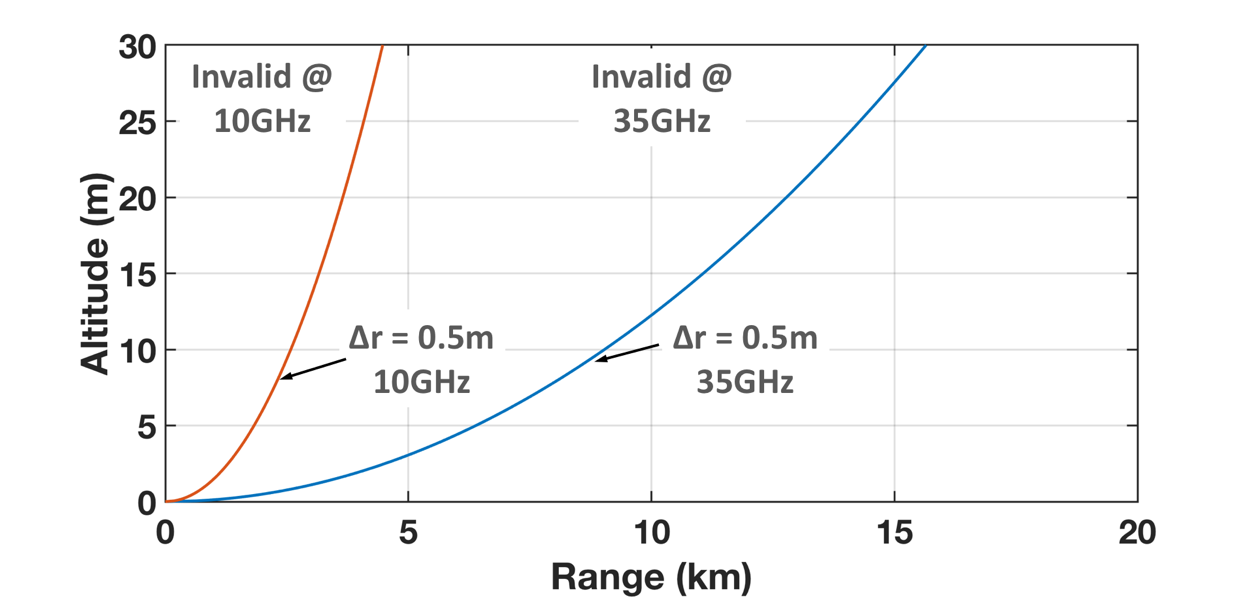
\includegraphics[width=5in]{../media/statistics/sampling_constraint.png}
  \end{center}
  \renewcommand{\baselinestretch}{1} \small\normalsize
  \begin{quote}
    \caption[Sampling Constraints for Statistical Analysis]{Sampling Constraints for Statistical Analysis\label{stat_fig:3}}
  \end{quote}
\end{figure}
\renewcommand{\baselinestretch}{2} \small\normalsize

\begin{figure}[H]
  \begin{center}
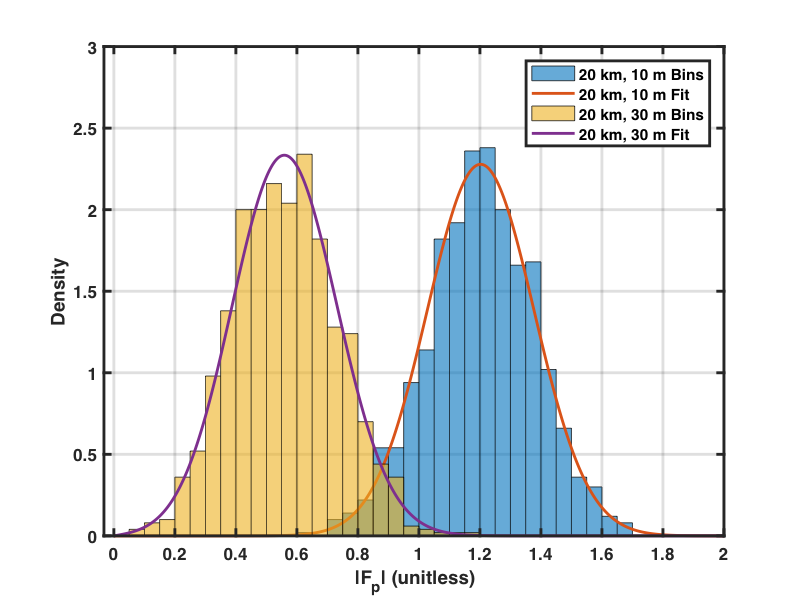
\includegraphics[width=5in]{../media/statistics/constant_range_fit.png}
  \end{center}
  \renewcommand{\baselinestretch}{1} \small\normalsize
  \begin{quote}
    \caption[PDF Fitting at Constant Range]{PDF Fitting at Constant Range\label{stat_fig:4}}
  \end{quote}
\end{figure}
\renewcommand{\baselinestretch}{2} \small\normalsize

\begin{figure}[H]
  \begin{center}
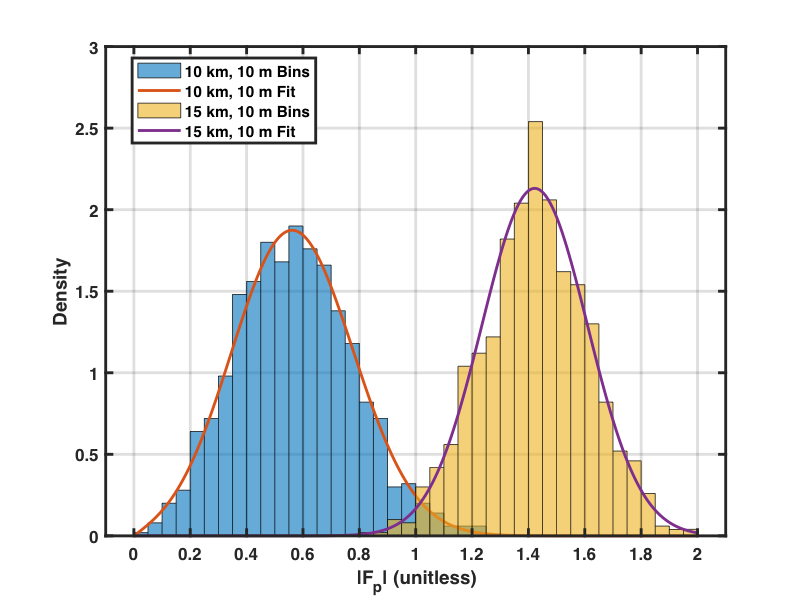
\includegraphics[width=5in]{../media/statistics/constant_altitude_fit.png}
  \end{center}
  \renewcommand{\baselinestretch}{1} \small\normalsize
  \begin{quote}
    \caption[PDF Fitting at Constant Altitude]{PDF Fitting at Constant Altitude\label{stat_fig:5}}
  \end{quote}
\end{figure}
\renewcommand{\baselinestretch}{2} \small\normalsize

\section{Configuration Geometry}
\section{One Way Path Results}
\section{Monostatic Results}
\section{Multistatic Results}